\documentclass[notitlepage,a4paper,oneside,article,table]{article}
\usepackage[utf8]{inputenc}
\usepackage{verbatim}
\usepackage[margin=1.0in]{geometry} %changes marges
\usepackage{minted} % src code highlighting: (https://www.overleaf.com/learn/latex/Code_Highlighting_with_minted)
\usemintedstyle{emacs} % code syntax highlighting style
\usepackage{amsmath}
\usepackage{amssymb}
\usepackage{fancyhdr}
\usepackage[dvipsnames]{xcolor}
\usepackage{pgfplots} 
\pgfplotsset{width=10cm, compat=1.9} %compat allows src code compilation
\usepgfplotslibrary{external} % speeds up compilation, we will externalize the figures
\tikzexternalize
\usepackage{graphicx}% allows the utilization of images
\graphicspath{ {./images/} }
\usepackage{placeins} %makes images stay in their own section/subsection, brilliant!
\usepackage[document]{ragged2e}
\usepackage{setspace}
\usepackage{tensor}
\usepackage{blindtext}
\usepackage{cancel}
\usepackage[dvipsnames]{xcolor}
\usepackage{fancyvrb}
\usepackage{pdfpages}
\usepackage{hyperref}
\usepackage{cancel}


\usepackage{listings}

\usepackage{xcolor}

%New colors defined below
\definecolor{codegreen}{rgb}{0,0.6,0}
\definecolor{codegray}{rgb}{0.5,0.5,0.5}
\definecolor{codepurple}{rgb}{0.58,0,0.82}
\definecolor{backcolour}{rgb}{0.95,0.95,0.92}

%Code listing style named "mystyle"
\lstdefinestyle{mystyle}{
  backgroundcolor=\color{backcolour}, commentstyle=\color{codegreen},
  keywordstyle=\color{magenta},
  numberstyle=\tiny\color{codegray},
  stringstyle=\color{codepurple},
  basicstyle=\ttfamily\footnotesize,
  breakatwhitespace=false,         
  breaklines=true,                 
  captionpos=b,                    
  keepspaces=true,                 
  numbers=left,                    
  numbersep=2pt,                  
  showspaces=false,                
  showstringspaces=false,
  showtabs=false,                  
  tabsize=2
}

%"mystyle" code listing set
\lstset{style=mystyle}

\hypersetup{
    colorlinks=true,
    linkcolor=violet,
    filecolor=Magenta,      
    urlcolor=blue,
    pdftitle={Overleaf Example},
    pdfpagemode=FullScreen,
    }
    
\urlstyle{same}
\newcommand\Perms[2]{\tensor[^{#2}]P{_{#1}}}

%#################################################################################################

\title{University of Houston - Clear Lake [Spring 2023] \\
CSCI 4336 - Introduction to Machine Learning\\
\colorbox{SkyBlue}{Logistic Regression using Java and Kaggle Titanic Dataset}}
\author{Student Name: Brandon E Ramirez}
\date{Date: 4/17/2023}

%Custom Macros:
\newcommand{\probP}{\text{I\kern-0.15em P}}
%End of custom macros

%used for importing txt files in proper format

% redefine \VerbatimInput
\RecustomVerbatimCommand{\VerbatimInput}{VerbatimInput}%
{fontsize=\footnotesize,
 %
 frame=lines,  % top and bottom rule only
 framesep=2em, % separation between frame and text
 rulecolor=\color{Gray},
 %
 label=\fbox{\color{Black} proposal.txt},
 labelposition=topline,
 %
}




\begin{document}

%header properties:
% Set the page style to "fancy"...
\pagestyle{fancy}
%... then configure it.

% Clear all headers and footers (see also \fancyhf{})
\fancyhead{}\fancyfoot{}

% Set the header and footer for Even
% pages but omit the zone (L, C or R)
\fancyhead[R]{Brandon E Ramirez}
\fancyhead[L]{CSCI 4336 – 01: Dr. Ahmed Abukmail}



\fancyfoot[L]{Logistic Regression using Java and Kaggle Titanic Dataset}
\fancyfoot[R]{Page No. \thepage}





\maketitle
\begin{center}
       \textbf{\colorbox{SpringGreen}{Assignment: Term Project}}\\   
       \vspace{0.2cm}
       \textbf{Due: 4/24/2023 @ 11:59PM}
       \vspace{0.2cm}\\
       \textsc{Student ID: 1952649}

\vspace{0.2cm}\\

\begin{figure}[h] % 'place image here (float)'
    \centering
    \includegraphics[width=0.25\textwidth]{images/logo.png}
\end{figure}
\FloatBarrier
       \newpage %pushes all the data to the next page
   \end{center}
\small \tableofcontents
\listoffigures
\vspace{1cm}

%be as detailed as you can and include many images, code, data, etc. (including email!)    

%****************************start document here**********************************
\section{Introduction}
The aim of this project is to implemnt the logistic regression machine learning algorithm using 
the Kaggle "Titanic - Machine Learning from Disaster" dataset. The model should be able to identify 
who survived the disaster by categorizing their likelyhood of survival as a 0 or 1. This will be based on the cummulative probability determined by the provided features. Surpassing a threshold value of $0.5$ or 50\% will output a logical 1 (survived), 0 (died) otherwise. 

\section{Project Scope/Requirements}
\includepdf[pages=1]{files/req.pdf}


\section{Email recap}

\verbatiminput{files/proposal.txt}

\section{Analyzing the data}
First of all, the training data was imported using Anaconda which was used to import dependencies and initialize Jupyter Notebook by using the cmd.exe prompt ("Jupyter Notebook"). The data was analyzed using a dataframe and was visualized using mathplotlib at this stage. I will use other tools to graph the Sigmoid function and the data's outputs later on. Here is my analysis of the data before cleaning it:\vspace{0.5cm}

Note* Further analytics about the data can be found at the source. Other files/data we will use are "gender\_submission.csv" which has a list of passenger ids and their actual survival outcome; and test.csv which we will use to verify the model later. 

%the pdf file starts here
\includepdf[pages=-]{files/2.pdf}

\includepdf[pages=-]{files/solarize.pdf}

\includepdf[pages=-]{files/data_scatter.pdf}


\iffalse 
Use this comment to keep track of references and work specific to this section
%**********************multi-line comment*****************************
https://tex.stackexchange.com/questions/105589/insert-pdf-file-in-latex-document

%*********************************************************************
\fi

\section{Cleaning the Data}
A machine learning model needs a good dataset in order to provide useful information. There are many ways to "prepare" or "clean" data, there may be fields that are incorrect, incomplete, irrelevant, duplicated, or improperly formatted.



\iffalse 
Use this comment to keep track of references and work specific to this section
%**********************multi-line comment*****************************
https://www.obviously.ai/post/data-cleaning-in-machine-learning
https://www.analyticsvidhya.com/blog/2021/10/handling-missing-value/
https://towardsdatascience.com/7-ways-to-handle-missing-values-in-machine-learning-1a6326adf79e

%*********************************************************************
\fi

   \subsection{Missing Values}
 While analyzing the excel data I noticed that there are missing values. A good approach to fix this is combing through each column and find which ones contain any missing values: PassengerId\{null\},Survived\{null\}, Pclass\{null\}, Name\{null\}, Sex\{null\}, SibSp\{null\}, Parch\{null\}, Ticket\{null\}, Fare\{null\}(some of the fares were 0 or free).
 
\begin{center}
    Age\{177 rows\}, Cabin\{206 rows\}, Embarked\{2 rows\}.
\end{center} 
 
 Some features don't matter or have data that a little to complex to interpret like cabin and ticket type, but the others must be free of error and have values to work with later on. The age column has the most missing values so I will concentrate on it. I can fill in these values by deleting the columns, inputting the mean as a placeholder value, or make an educated guess as to what the passengers likely paid. I will do a combination of these three. For a third of the passengers I will assign them an age based on the price of their ticket in the following way:


\begin{center}
\begin{tabular}{ |c|c|c| } 
 \hline
Avg Ticket cost & Range & Projected Age\\
 \hline
 $\leq$ \$35(£7) & 0-20 & 10 \\ 
  \hline
 \$35 $\leq$ \$65(£12) & 20-45 & 30 \\ 
  \hline
 \$65 $\leq$ \$400(£30)  & 45+ & 55 \\ 
 \hline
\end{tabular}
\end{center}

I will assign \textcolor{red}{50} missing ages using this method, assign \textcolor{blue}{50} the mean age (29.699118 $\approx$ 30), and remove the remaining rows with missing values. These will be colored differently in the excel training data file. We now have 814 rows to train the model with. Source: \url{https://rmstitanic1912.weebly.com/the-cost-of-tickets.html}



    \subsection{Interpreting the Features}
The "embarked" feature has 3 letters denoting the ports of embarkation, C = Cherbourg, Q = Queenstown, S = Southampton. The embarked column only has 2 missing values so I will just make an educated guess with those based on ticket price and port. Finally, I will be marking them as 0,1, or 2 based on the relative GDP of each town in 1912 (C=0,S=1,Q=2) where "3" was the wealthiest port at the time. This feature may not be useful enough as the port cities might not hold sufficient applicable information to get any practical results. The sex of each passenger can be interpreted as 0 for male and 1 for female. 

    \subsection{Useful features}

We need to make an assessment of which features are quantifiable and relevant to our model. We have a decent collection of features to work with but we need to choose the features that will grant us useful results. The columns that are seemingly unnecessary are cabin, name, and ticket number; these features should have no effect on our results. There is also the matter of extrapolating useful information from the remaining columns. PassengerId will be used to identify a passenger (1 to 814), and "survived" are essential to managing and testing the model. We need to scrutinize the features and possibly omit/include them to revise the model as we see fit. The features we will definitely use are: sex, age, fare, Pclass, SibSp, Parch, \& embarked.
    
\section{How Binomial Logistic (logit) Regression Works}
\iffalse 
Use this comment to keep track of references and work specific to this section
%**********************multi-line comment*****************************
https://medium.com/@zaxxio/build-neural-network-in-java-c3dde0ab8887

%*********************************************************************
\fi
Logistic regression uses the sigmoid function which is a mathematical function used to assign predicted values to probabilities by mapping any real value into another value within a range of 0 to 1. It is defined by a characteristic S-shaped curve or sigmoid curve which is produced as y values asymptotically approach 0 and 1 as the x values approach $-\infty$ and $\infty$ respectively. The input weights/parameters must be trained to this curve best-fits our dataset. Once the curve reasonably approximates our dataset we can start making useful predictions. Some assumptions about the data are:\\
\begin{enumerate}
    \item   The dependent variable must be categorical in nature
    \item   Only relevant variables should be included
    \item   Large sample size is required
    \item   The independent variable should not have multi-collinearity
    \item   Given output $\hat{y}$, if $\hat{y} \geq 0.5$ then output $= O(1)$, else $\hat{y} < 0.5 = O(0)$
\end{enumerate}

\begin{figure}[h] % 'place image here (float)'
    \centering
    \includegraphics[width=.75\textwidth]{how/lr.png}
    \caption{High Level Logistic Regression Schematic}
\end{figure}
\FloatBarrier

\begin{center}
   The above process can be described mathematically as: "$y = w_{1}\cdot x_{1} + w_{2}\cdot x_{2} + w_{3}\cdot x_{3} + \ldots + w_{n-1}\cdot x_{n-1} + w_{n}\cdot x_{n} + b$" or $y = w^{T}x + b$". If $\hat{y} \geq 0.5 = O(1)$, else $\hat{y} < 0.5 = O(0)$
\end{center}
\vspace{0.125cm}

This is another way of writing it: \\
$$
\begin{bmatrix}
x_{1}, &
x_{2}, &
x_{3}, &
$\ldots$, &
x_{n-1}, &
x_{n}
\end{bmatrix}_{1 \times n}
\cdot
\begin{bmatrix}
w_{1},\\
w_{2},\\
w_{3},\\
$\ldots$,\\
w_{n-1}, \\
w_{n}
\end{bmatrix}_{n \times 1}
+ b
\rightarrow
N
\rightarrow
A
\rightarrow
U
\rightarrow
O(0,1)
$$

\begin{center}
    Where b = bias term, N = Net Input Function, A = Activation Function, U = Unit Step Function, O = Output.
\end{center}

The $x$ row vector are the input features, the $w$ column vector are the weights which are initialized to 0 when we begin training the model.


\vspace{0.5cm}
The logistic regression algorithm needs several components, these include:

\begin{enumerate}
    \item Sigmoid function (activation function)\\

    $$\sigma(x) = \frac{1}{1 + e^{-x}} = \frac{e^{x}}{e^{x} + 1}$$
\begin{center}
    where $\sigma(x) =$ S(x) =  sigmoid function, e = Euler's Number ($\approx$ 2.71828)\\
Domain: ($-\infty, \infty$), Range: (0, +1), \& S(0) = 0.5    
\end{center}

\begin{figure}[h] % 'place image here (float)'
    \centering
    \includegraphics[width=0.5\textwidth]{how/1.png}
    \caption{Sigmoid function}
\end{figure}
\FloatBarrier

\begin{figure}[h] % 'place image here (float)'
    \centering
    \includegraphics[width=0.5\textwidth]{how/dis&con.png}
    \caption{The sigmoid function can give us a continous value (probability) as well as a discrete value.}
\end{figure}
\FloatBarrier

    \item Cost function\\
    The cost function is a representation of the error in our predictions, we need to decrease its value in order to get accurate results. 
    $$\hat{y} = \sigma(w^{T}x+b) = \frac{1}{1+e^{-w^{T}x+b}}$$
    $$cost = \frac{-1}{m} \cdot \sum_{i=o}^{m} [y \cdot log(\hat{y}) + (1 - y)log(1-\hat{y})]$$
    Where m = number of values in the data-set, $\hat{y}$ is our predicted value, and $y$ is the actual value. We use this function because it only allows for 0 or 1 (or any range in between) to be accepted values. Lets see what happens when y equals 0 and 1 for a single observation:

    \begin{equation}
  \text{if } y = \begin{cases}
    1, & \text{error $= -log(\hat{y})$}; \text{because:} -[y \cdot log(\hat{y}) + \cancelto{0}{(1 - y)log(1-\hat{y})} ]\\

    0, & \text{else, error $= -log(1 - \hat{y})$}; \text{because:} -[\cancelto{0}{(y \cdot log(\hat{y}))} + (1 - y) \cdot log(1-\hat{y})]
  \end{cases}
\end{equation}

If the true value $y = 1$, and our predicted value $\hat{y}$ is close or equal to 1, then the error rate will be lower because $-log(1)=0$. 
Otherwise, if the true value $y = 0$, and our predicted value $\hat{y}$ is close or equal to 0, then the error rate will be lower because $-log(1)=0$.




\begin{figure}[h] % 'place image here (float)'
    \centering
    \includegraphics[width=1\textwidth]{how/cost.png}
    \caption{Cost function behavior when y = 1, \& y = 0}
\end{figure}
\FloatBarrier

    
    \item Gradient descent\\
    Gradient descent is an iterative optimization algorithm which will help us reduce the cost function value by modifying the weight(s) in our model so that we can approach a global minima. This part of the algorithm will be repeated using a for loop. This algorithms components are:
    $$\hat{W} = W - \alpha \cdot \frac{\partial_{cost}}{\partial_{W}}$$
    $$\hat{b} = b - \alpha \cdot \frac{\partial_{cost}}{\partial_{b}}$$
    \\
    The first order derivatives can also be written as: 
	
    $$\frac{\partial_{cost}}{\partial_{W}} = (\hat{y} - y) \cdot x$$
    $$\frac{\partial_{cost}}{\partial_{b}} = (\hat{y} - y)$$
    $$\therefore \hat{W} = W - \alpha \cdot \boldsymbol{(\hat{y} - y) \cdot x}$$
    $$\hat{b} = b - \alpha \cdot \boldsymbol{(\hat{y} - y)}$$
    \begin{center}
    s.t. $\alpha = $ learning rate, $\hat{W} = $ the new weight, $\hat{b} = $ is the updated y intercept. The bold $\hat{y}, y, x$ represent the matrix form of all utilized observations in data-set.
    \end{center}
    \\
    The type of gradient descent I will use is batch gradient descent, which calculates the error for each example within the training data-set. The model is not revised until every training sample has been assessed. Every cycle is referred to as a cycle or a training epoch. The learning rate hyper-parameter must be chosen to avoid surpassing the global minima along the x-axis but not be too small so that it doesn't take too many iterations to find it.

    \begin{figure}[h] % 'place image here (float)'
    \centering
    \includegraphics[width=0.5\textwidth]{how/slope.png}
    \caption{The rate of error is minimized as the slope approaches $0$}
\end{figure}
\FloatBarrier

    \begin{figure}[h] % 'place image here (float)'
    \centering
    \includegraphics[width=0.75\textwidth]{how/new_gd.png}
    \caption{Optimization of logistic curve}
\end{figure}
\FloatBarrier
    
\end{enumerate}


\section{Source Code \& Technical Challenges}
\subsection{My code}
The code for this project is in the folder X, just open the file from any IDE including the data-sets files to run the program. 



\subsection{Explanation}
The program should be able to generate a list of outputs including the cost function value after a certain number of epochs as well as the rate of success once the model has been fully trained.

\subsection{Processing the Data}
The data needs to be stored in a way such that all the relevant data can be called when needed and to 
run analysis on it (margin of error, etc.). The data must be able to read the train-X(gives us id and other features) and train-Y data (tells us who survived as well as id). The way in which the algorithm is implemented should be easy to replicate using Python and Jupyter Notebooks like in the SciKit Learn book. I deleted the header rows for each file to get them out of the way of calculations. I then took the transpose of the input matrix so that each feature could be read as an individual line into Java. I had difficulty importing the csv data so I converted them to txt files and used the following code to read from the files at specific lines so I could give them the appropriate feature names and save them in their easy to access array format.

\begin{lstlisting}[language=Java, caption=Importing the rows from external files]
import java.nio.file.Files;
import java.nio.file.Paths;
//          ...
String test_X_embarked = Files.readAllLines(Paths.get(test_X)).get(7);
\end{lstlisting}

I then had to parse these string arrays to either integer or float arrays. After I had done this for all the files I could finally start training the model


\subsection{Tech Stack Used}

The project needed the use Java, my IDE of choice was IntelliJ IDEA. 
I planned using the Java 2D Graphics API provided by Oracle. I realized awt + swing is used for creating GUI components rather than for plotting and visualizing data. 

\subsection{Visualizing the data (optional)}

The probability(x) should be mapped to a function $\sigma$(x) which will yield a y-axis value, this can be used to visualize the coordinate points. Ideally, by pressing the coordinate point it should display the calculated probability and whether or not they survived as well as age, sex, name, \& whether or not they actually survived. I decided to do this later on and not visualize the data this time. I plan to do it later.

\subsection{Results}
Our rate of success was should be in the program output. I'm sure we could improve our results by including observations from the other data-sets, using other techniques (stochastic gradient descent, etc.) or experimenting with the "iterations" and "learning rate" parameters further. Feel free to experiment with the parameters and try to find the sweet spot yourself.

%\subsection{Margin of Error}The error was calculated using this code:

%%\end{lstlisting}





\section{Running My Logistic Regression Algorithm (Instructions)}
Just make sure to read the "READ$_$ME".txt file that came int the Java source folder. It should be simple since running the program doesn't require setting up any external dependencies. There shouldn't be any setting up on your part to make it work, everything is set to just run.

\section{SciKitLearn Textbook Implementation}
The book "Hands-On Machine Learning with Scikit-Learn, Keras, and TensorFlow" talks about logistic regression on page 268 using the famous Iris data-set. It primarily uses the sklearn "LogisticRegression" and "train-test-split" python classes from the model selection and linear modules to train and process the model. 

%\url{https://scikit-learn.org/stable/modules/generated/sklearn.linear_model.LogisticRegression.html}

\subsection{SciKit Source Code}
%\includepdf[pages=-]{files/SkLearn_Logistic_Regression.pdf}
\begin{lstlisting}[language=Python, caption=Code used in book using Titanic dataset]
#!/usr/bin/env python
# coding: utf-8
# In[1]:
import numpy as np
import pandas as pd
from sklearn.model_selection import train_test_split
from sklearn.linear_model import LogisticRegression
from sklearn.metrics import accuracy_score
titanic_data = pd.read_csv('train.csv')
# In[2]:
# check the number of missing values in each column
titanic_data.isnull().sum()
# In[3]:
# drop the "Cabin" column from the dataframe
titanic_data = titanic_data.drop(columns='Cabin', axis=1)
# In[4]:
# replacing the missing values in "Age" column with mean value
titanic_data['Age'].fillna(titanic_data['Age'].mean(), inplace=True)
# In[5]:
# replacing the missing values in "Embarked" column with mode value
titanic_data['Embarked'].fillna(titanic_data['Embarked'].mode()[0], inplace=True)
# In[6]:
# converting categorical Columns
titanic_data.replace({'Sex':{'male':0,'female':1}, 'Embarked':{'S':0,'C':1,'Q':2}}, inplace=True)
# In[7]:
X = titanic_data.drop(columns = ['PassengerId','Name','Ticket','Survived'],axis=1)
Y = titanic_data['Survived']
print(X)
# In[8]:
print(Y)
# In[9]:
X_train, X_test, Y_train, Y_test = train_test_split(X,Y, test_size=0.2, random_state=2)
# In[10]:
print(X.shape, X_train.shape, X_test.shape)
# In[11]:
#Training the model using Logistic Regression
model = LogisticRegression()
# training the Logistic Regression model with training data
model.fit(X_train, Y_train)
# In[12]:
# accuracy on training data
X_train_prediction = model.predict(X_train)
print(X_train_prediction)
# In[13]:
training_data_accuracy = accuracy_score(Y_train, X_train_prediction)
print('Accuracy score of training data : ', training_data_accuracy)
\end{lstlisting}
\subsection{Results \& Comparison}

\begin{figure}[h] % 'place image here (float)'
    \centering
    \includegraphics[width=0.75\textwidth]{code/1.png}
\end{figure}
\FloatBarrier


\section{Conclusion}

Logistic regression is a statistical technique used to model the probability of a binary response variable based on one or more predictor variables. It is a type of regression analysis that uses a logistic function to transform the output of a linear regression model into a probability value between 0 and 1. The model estimates the coefficients of the predictor variables, which are used to calculate the odds of the response variable being in one category over the other. Logistic regression is widely used in various fields, including medicine, economics, and social sciences, to predict the probability of outcomes such as disease diagnosis or customer behavior.


\section{Appendices}
\textcolor{red}{N/A}

\section{Sources}

Data
\begin{enumerate}
    \item \url{https://www.kaggle.com/competitions/titanic/data}
\end{enumerate}

Math and Algorithm Reference
\begin{enumerate}
    \item \url{https://www.analyticsvidhya.com/blog/2022/07/gradient-descent-and-its-types/}
    \item \url{https://www.javatpoint.com/logistic-regression-in-machine-learning}
\end{enumerate}

General LaTeX reference: 

\begin{enumerate}
    \item \url{https://www.math.uci.edu/~xiangwen/pdf/LaTeX-Math-Symbols.pdf}
    \item \url{https://www.overleaf.com/learn/latex/Learn_LaTeX_in_30_minutes}
    \item \url{https://www.youtube.com/watch?v=ydOTMQC7np0}
\end{enumerate}

Excel Reference:
\begin{enumerate}
    \item \url{https://www.youtube.com/watch?v=YiC-z_FH7SU}
    \item \url{https://www.youtube.com/watch?v=fSLBEPJglaU}
\end{enumerate}

Code formatting and colors reference: \url{https://www.overleaf.com/learn/latex/Code_listing}\\
Colors reference: \url{https://www.overleaf.com/learn/latex/Using_colours_in_LaTeX}\\
Java 2D Graphics API Documentation: \url{https://docs.oracle.com/javase/tutorial/2d/index.html}\\

Other Documentation:
\begin{enumerate}
    \item \url{https://nbconvert.readthedocs.io/en/latest/install.html}
    \item \url{https://www.dunderdata.com/blog/view-all-available-matplotlib-styles}
    \item \url{https://texdoc.org/serve/pdfpages/0}
    \item \url{https://www.overleaf.com/learn/latex/Matrices}
\end{enumerate}

SciKit Learn:
\begin{enumerate}
    \item \url{https://scikit-learn.org/stable/modules/generated/sklearn.linear_model.LogisticRegression.html#sklearn.linear_model.LogisticRegression}
\end{enumerate}


\vspace{0.5cm}

Miscellaneous Sources:
\begin{enumerate}
    \item \url{https://stackoverflow.com/questions/2739159/inserting-a-pdf-file-in-latex}
    \item \url{https://tex.stackexchange.com/questions/85200/include-data-from-a-txt-verbatim}
    \item \url{https://www.overleaf.com/learn/latex/Headers_and_footers}
    \item \url{https://stackoverflow.com/questions/4027363/two-statements-next-to-curly-brace-in-an-equation}
    \item \url{https://jansoehlke.com/2010/06/strikethrough-in-latex/}
\end{enumerate}

Tools:
\begin{enumerate}
    \item \url{(ChatGPT, personal communication, April 22, 2023)}
    \item \url{https://www.tablesgenerator.com/}
    \item \url{https://htmtopdf.herokuapp.com/ipynbviewer/}
    \item \url{https://phrasefix.com/tools/remove-tabs-from-text/}
\end{enumerate}



Other: 
\begin{enumerate}
    \item \url{https://en.wikivoyage.org/wiki/RMS_Titanic}
    
\end{enumerate}

% Use the resources below to help prepare this document

\iffalse 
Use this comment to keep track of references and work specific to this section
%**********************multi-line comment*****************************


%*********************************************************************
\fi

\iffalse 
\begin{figure}[h] % 'place image here (float)'
    \centering
    \includegraphics[width=1\textwidth]{}
    \caption{}
\end{figure}
\FloatBarrier
\fi

\end{document}




